\section{Bdd}

\begin{flushleft}
Au niveau de la base de données, j'ai besoin dans un premier temps de stocker plus d'informations sur l'habitation des clients, c'est-à-dire dans la table \textbf{portefeuille}. Notamment le nombre de personnes habitant dans cette dernière, le type de maison, le type de chauffage et finalement s'il y a une présence de panneaux solaires.
\end{flushleft}

\begin{flushleft}
Dans un second temps, j'ai stocké les données de consommations qui serviront de comparaison. Pour cela, une nouvelle table a été crée, à savoir \textbf{consommation de simulation}. Nous devons donc y retrouver des données de consommations, un type d'énergie et une date mais il faut aussi pouvoir les distinguer en fonction des caractéristiques de la maison, c'est pourquoi nous y retrouvons également les mêmes types de données que dans la table portefeuille. C'est-à-dire le nombre d'habitants, le type de maison, le type de chauffage et s'il y a des panneaux solaires.
\end{flushleft}

\begin{figure}[h]
\centering
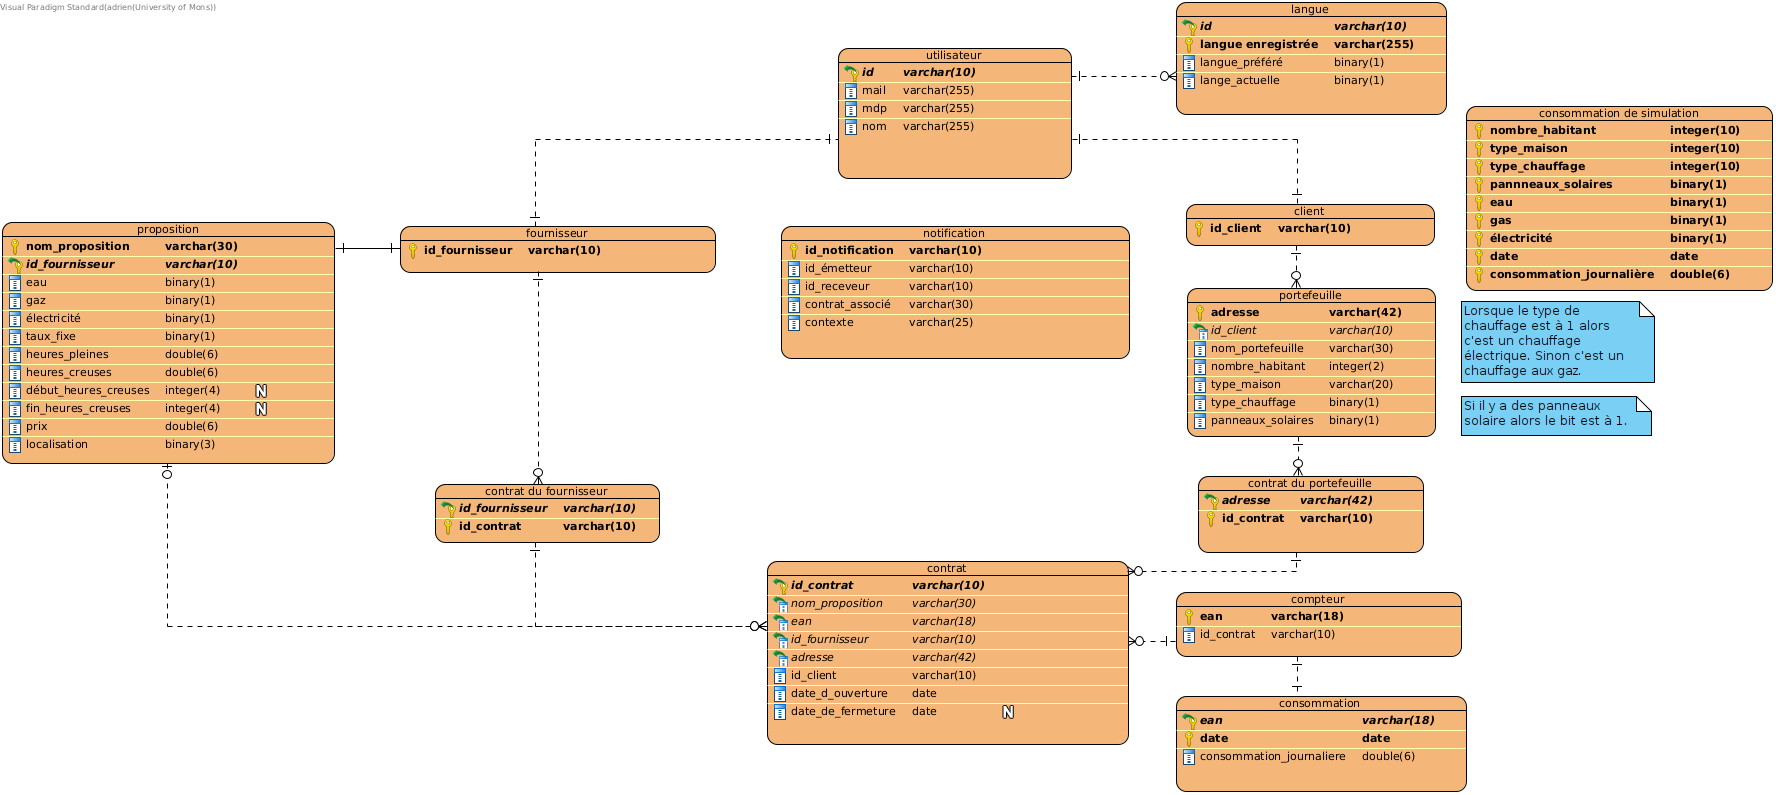
\includegraphics[width=1.3\textwidth]{extension-adrien/Bdd/img/bdd.png}
\end{figure}
